\documentclass{article}
\usepackage{graphicx} % Required for inserting images
\usepackage{amssymb}
\usepackage{hyperref}
\hypersetup{
    colorlinks=true,
    linkcolor=blue,
    filecolor=magenta,      
    urlcolor=cyan,
    pdftitle={Overleaf Example},
    pdfpagemode=FullScreen,
    }

\urlstyle{same}
\usepackage{booktabs}

\title{CSE590 Project 1}
\author{Michael Karen, Pouya Karimiandehaghi}
\date{March 2026}

\begin{document}

\maketitle

\section{Introduction}

This project involved the design, simulation, and hardware synthesis of a simple single-cycle, non-pipeline 16-bit processor. The processor follows a MIPS-inspired architecture, scaled to 16 bits. Our design has 8 main components: Program Counter, Instruction Memory, Register File, ALU, Sign Extender, Data Memory, Control Unit, and Multiplexers.


\section{Data Path}

The data path for our design is shown in Figure \ref{fig:datapath}.

\begin{figure}[htbp]
    \centering
    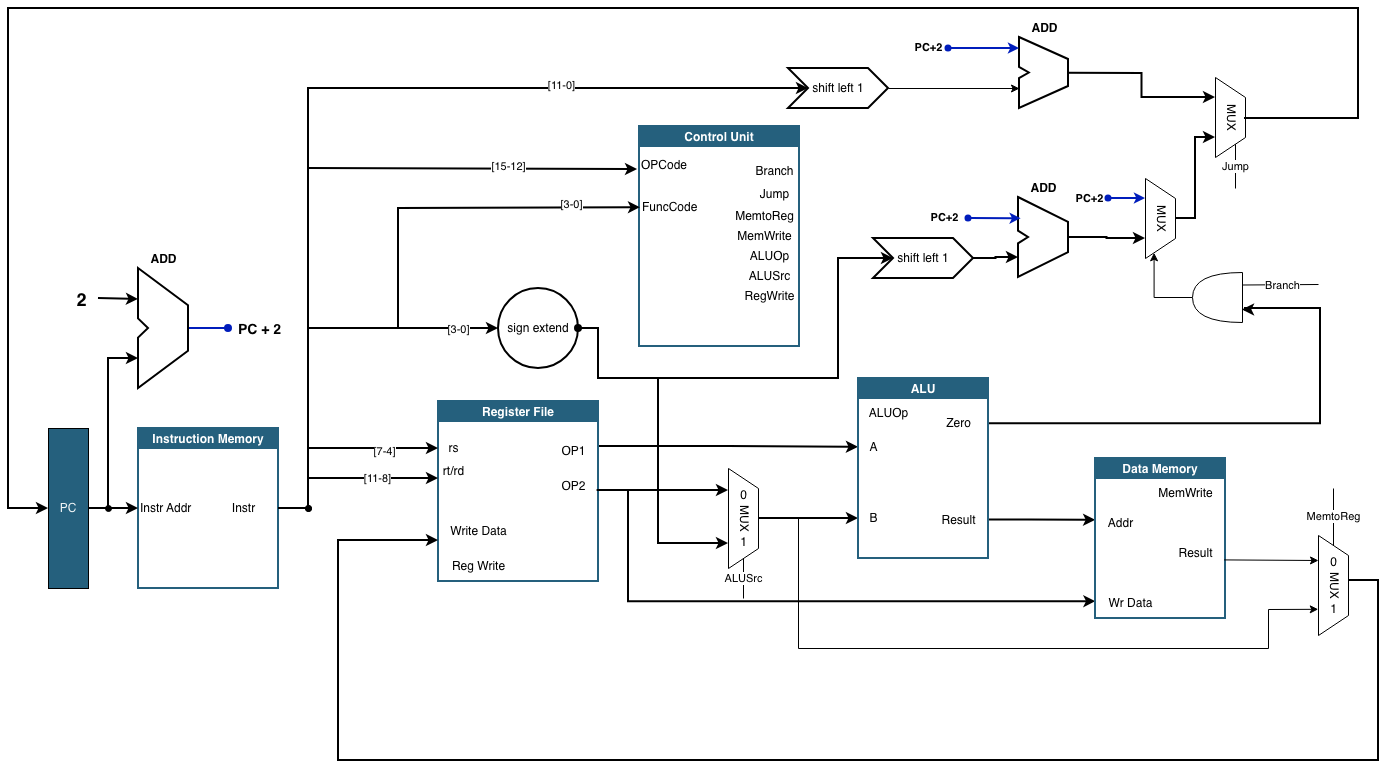
\includegraphics[width=0.8\linewidth]{data_path_final.png}
    \caption{Data path design for the single-cycle non-pipeline 16-bit processor}
    \label{fig:datapath}
\end{figure}

\section{Modules}


\subsection{Program Counter}

The Program Counter (PC) stores the address of the current instruction and updates it every clock cycle to point to the next instruction. In this processor, the PC typically increments by 2 because each instruction is 16 bits (2 bytes). The PC may also be updated by branch or jump logic depending on control signals generated by the Control Unit. In the Verilog implementation, this functionality is implemented in \texttt{PC.v}, which contains the current instruction address and updates it on the clock edge.


\subsection{Instruction Memory}

The Instruction Memory stores the program instructions and outputs the instruction corresponding to the address provided by the Program Counter. When the PC sends an address, the instruction memory returns the 16-bit instruction stored at that location. This instruction is then decoded and used by the rest of the datapath. The instruction memory is integrated within the top-level processor design, mainly managed in \texttt{Processor\_Wrapper.v}, where instructions are fetched using the PC address.

\subsection{Register File}

The Register File stores the processor registers and provides operands for ALU operations. It supports reading two registers simultaneously and writing a result back to a register when the write-enable signal is asserted. In this implementation, the register access and operand extraction are handled inside \texttt{Decoder.v}. The decoder parses the instruction fields (such as \texttt{rs} and \texttt{rt/rd}), reads the corresponding register values, and outputs the operands (\texttt{op1\_o} and \texttt{op2\_o}) that are later used by the ALU. It also supports writing results back into registers when \texttt{reg\_wen} is asserted.


\subsection{Sign Extension}

The Sign Extension unit converts the smaller immediate value present in I-type instructions into a full 16-bit signed value so it can be used in arithmetic operations or memory address calculations. In this implementation, the immediate value extracted from the instruction is produced by \texttt{Decoder.v} (output \texttt{imm\_o}) and then used by the execution stage.


\subsection{Control Unit}
The Control Unit determines the behavior of the processor based on the instruction opcode and function code. It generates control signals that determine ALU operations, memory access, register writes, and branching behavior. The control logic is implemented in \texttt{Controller.v}, which interprets the instruction type and produces signals such as \texttt{Branch}, \texttt{Jump}, \texttt{MemtoReg}, \texttt{MemWrite}, \texttt{ALUSrc}, and \texttt{RegWrite}. The instruction fields needed for this control logic are extracted by \texttt{Decoder.v}, which separates the opcode and function fields from the instruction.

The file \texttt{Defines.v} contains global macro definitions used throughout the processor design. These definitions include opcode values for instructions (such as \texttt{OP\_LW}, \texttt{OP\_SW}, \texttt{OP\_ADDI}, and \texttt{OP\_JMP}), function codes for R-type instructions (such as \texttt{FUNCT\_ADD} and \texttt{FUNCT\_SUB}), and ALU operation codes. By centralizing these constants in \texttt{Defines.v}, the design ensures consistency across modules such as \texttt{Decoder.v}, \texttt{Controller.v}, and the execution logic while improving code readability and maintainability.


\subsection{ALU}

The Arithmetic Logic Unit (ALU) performs arithmetic and logical operations such as addition, subtraction, shift-left, and bitwise AND. It takes two operands from the register file or immediate values and produces the result used either for writing back to registers or accessing memory. The ALU also generates a \texttt{Zero} signal used for branch decisions. The ALU functionality is implemented within the execution stage in \texttt{Execute.v}.

\subsection{Multiplexers}

Multiplexers (MUXes) are used throughout the datapath to select between multiple input sources. For example, a MUX selects whether the ALU receives a register value or an immediate value using the \texttt{ALUSrc} control signal. Another MUX selects whether the value written back to the register file comes from the ALU or from memory using the \texttt{MemtoReg} signal. Additional multiplexers determine the next PC value during branch or jump instructions. These multiplexing operations are implemented inside the datapath logic in \texttt{Execute.v} and coordinated by control signals generated in \texttt{Controller.v}.

\subsection{Data Memory}

The Data Memory stores data used by load (\texttt{lw}) and store (\texttt{sw}) instructions. When a load instruction occurs, the memory outputs the data stored at the computed address, and when a store instruction occurs, the data from a register is written into memory. Memory access is controlled using signals such as \texttt{MemWrite}. The memory behavior is implemented in \texttt{DataMemory.v}, which models the memory as an array and handles both read and write operations.

\section{Contributions and GitHub}
Github repository link:
\url{https://github.com/MichaelCKaren/CSE590\_ProcessorProject1\_MK\_PK\_JL.git}

\begin{table}[h]
  \caption{Task Distributions.}
  \label{tab:results}
  \centering
  \begin{tabular}{lccc} % l=left aligned, c=centered
    \toprule
    Tasks & Michael Karen & Pouya Karimiandehaghi & Jiadong Liang \\
    \midrule
    Datapath & \checkmark & \checkmark &  \\
    Code structure & \checkmark  &  &  \\
    Program Counter & \checkmark & \checkmark  &  \\
    ADD & \checkmark &  &  \\
    SUB &  &  & \checkmark \\
    SLL &  &  & \checkmark \\
    AND &  &  & \checkmark \\
    ADDI &  & \checkmark &  \\
    SW  & \checkmark &  &  \\
    LW  &  & \checkmark &  \\
    BEQ &  & \checkmark &  \\
    BNE & \checkmark &  &  \\
    JMP & \checkmark &  &  \\ 
    Report &  & \checkmark & \checkmark \\
    \bottomrule
  \end{tabular}
\end{table}


\begin{table}[htbp]
  \caption{Weekly logs.}
  \label{tab:results}
  \centering
  \begin{tabular}{lp{0.7\linewidth}} % l=left aligned, c=centered
    \toprule
    Date & Details \\
    \midrule
    23\textsuperscript{rd} February & Group formation and registration \\
    3\textsuperscript{rd} March & Discussed about project structure and started the Github repository \\
    6\textsuperscript{th} March & Discussed data path \\
    12\textsuperscript{th} March & Drew the first version of data path \\
    13\textsuperscript{th} March& Finalized the data path, code structure, program counter, ADD and task distribution \\
    14\textsuperscript{th} March& Finalized the checkpoint submission \\
    \bottomrule
  \end{tabular}
\end{table}

\end{document}
